\documentclass[12pt,norsk,a4paper]{article}
\usepackage[norsk]{babel}
\usepackage[norsk]{isodate}
\usepackage[T1]{fontenc}
\usepackage{parskip}
\usepackage{url}
\usepackage{cancel}
\usepackage{mathtools}
\usepackage{xfrac}
\usepackage{listings}
\author{Frida Berge (fridatbe)}
\title{IN3140 --- Obligatorisk oppgave 1}
\date{\today}
\usepackage[small,euler-digits]{eulervm}
\usepackage{color}
% \usepackage{minted}
\usepackage{xcolor}
\definecolor{LightGray}{gray}{0.9}
\usepackage{a4wide}
\usepackage[top=2cm]{geometry}
\usepackage{graphicx}
\graphicspath{ {./fig/} }
\newcommand{\tuple}[1]{\ensuremath{\langle #1\rangle}}
\newcommand{\set}[1]{\ensuremath{\{#1\}}}
\newcommand{\imp}{\ensuremath{\rightarrow}}
\newcommand{\M}{\ensuremath{\mathcal{M}}}
\newcommand{\AF}{edge from parent[draw=none]}
\newcommand{\NODE}[1]{\{node \{\ensuremath{#1}\}\}}
\usepackage[explicit]{titlesec}
\titleformat{\section}{\normalfont\Large\bfseries}{}{0em}{#1\ \thesection}


\begin{document}
    \maketitle
    \renewcommand{\thesubsection}{(\alph{subsection})}
    \newpage

    \section{Task}
    \textbf{1a)}\\
    Finding the transformation matrix expressing the position and orientation of T with respect to B ($T_T^{B}$):
    
        \[T_T^{B} = 
            \left[ \begin{array}{cc}
                R_T^B & d_t^B \\
                0 & 1\\
            \end{array} \right]\]

        Finding the rotation matrix $R_T^B$:
        \[R_T^{B} = \left[ \begin{array}{ccc}
            c\frac{\pi}{2} & -s\frac{\pi}{2} & 0 \\
            s\frac{pi}{2} & c\frac{pi}{2} & 0 \\
            0 & 0 & 1 \\
        \end{array} \right]
        =\left[ \begin{array}{ccc}
            0 & -1 & 0 \\
            1 & 0 & 0 \\
            0 & 0 & 1 \\
        \end{array} \right]\]

        Finding the translation matrix $d_T^B$:
        \begin{itemize}
            \item Translation in $x_B$-direction is defined as $-y_w$-direction (since they are parallel and pointed in opposite direction). 
            So the translation from $O_B$ to $O_T$ in x-direction relative to coordinate system B 
            is based in the y-coordinates in Figure 2.
            And therefore the translation from B to T in y-direction is: -(400 - 650) = \underline{250}
            \item In the same way we can see that translation in $y_B$ direction correspond to $-x_w$.
            So translation from $O_B$ to $O_T$ in y-direction is: -(1000 - 250) = \underline{-750}
            \item The translation in $z_B$-direction is correspond to $-z_w$-direction.
            So the translation from $O_B$ to $O_T$ inn z-direction is: -(900 - 1000) = \underline{100}
        \end{itemize}


        \[d_T^{B}
        =\left[ \begin{array}{c}
            250 \\
            -750 \\
            100 \\
        \end{array} \right]\]
        The total homogeneous transformation:
        \[T_T^{B} = 
            \underline{\left[ \begin{array}{cccc}
                0 & -1 & 0 & 250 \\
                1 & 0 & 0 & -750 \\
                0 & 0 & 1 & 100 \\
                0 & 0 & 0 & 1 \\
            \end{array} \right]}\]
    
    \section{Task}
    \textbf{2a)}
    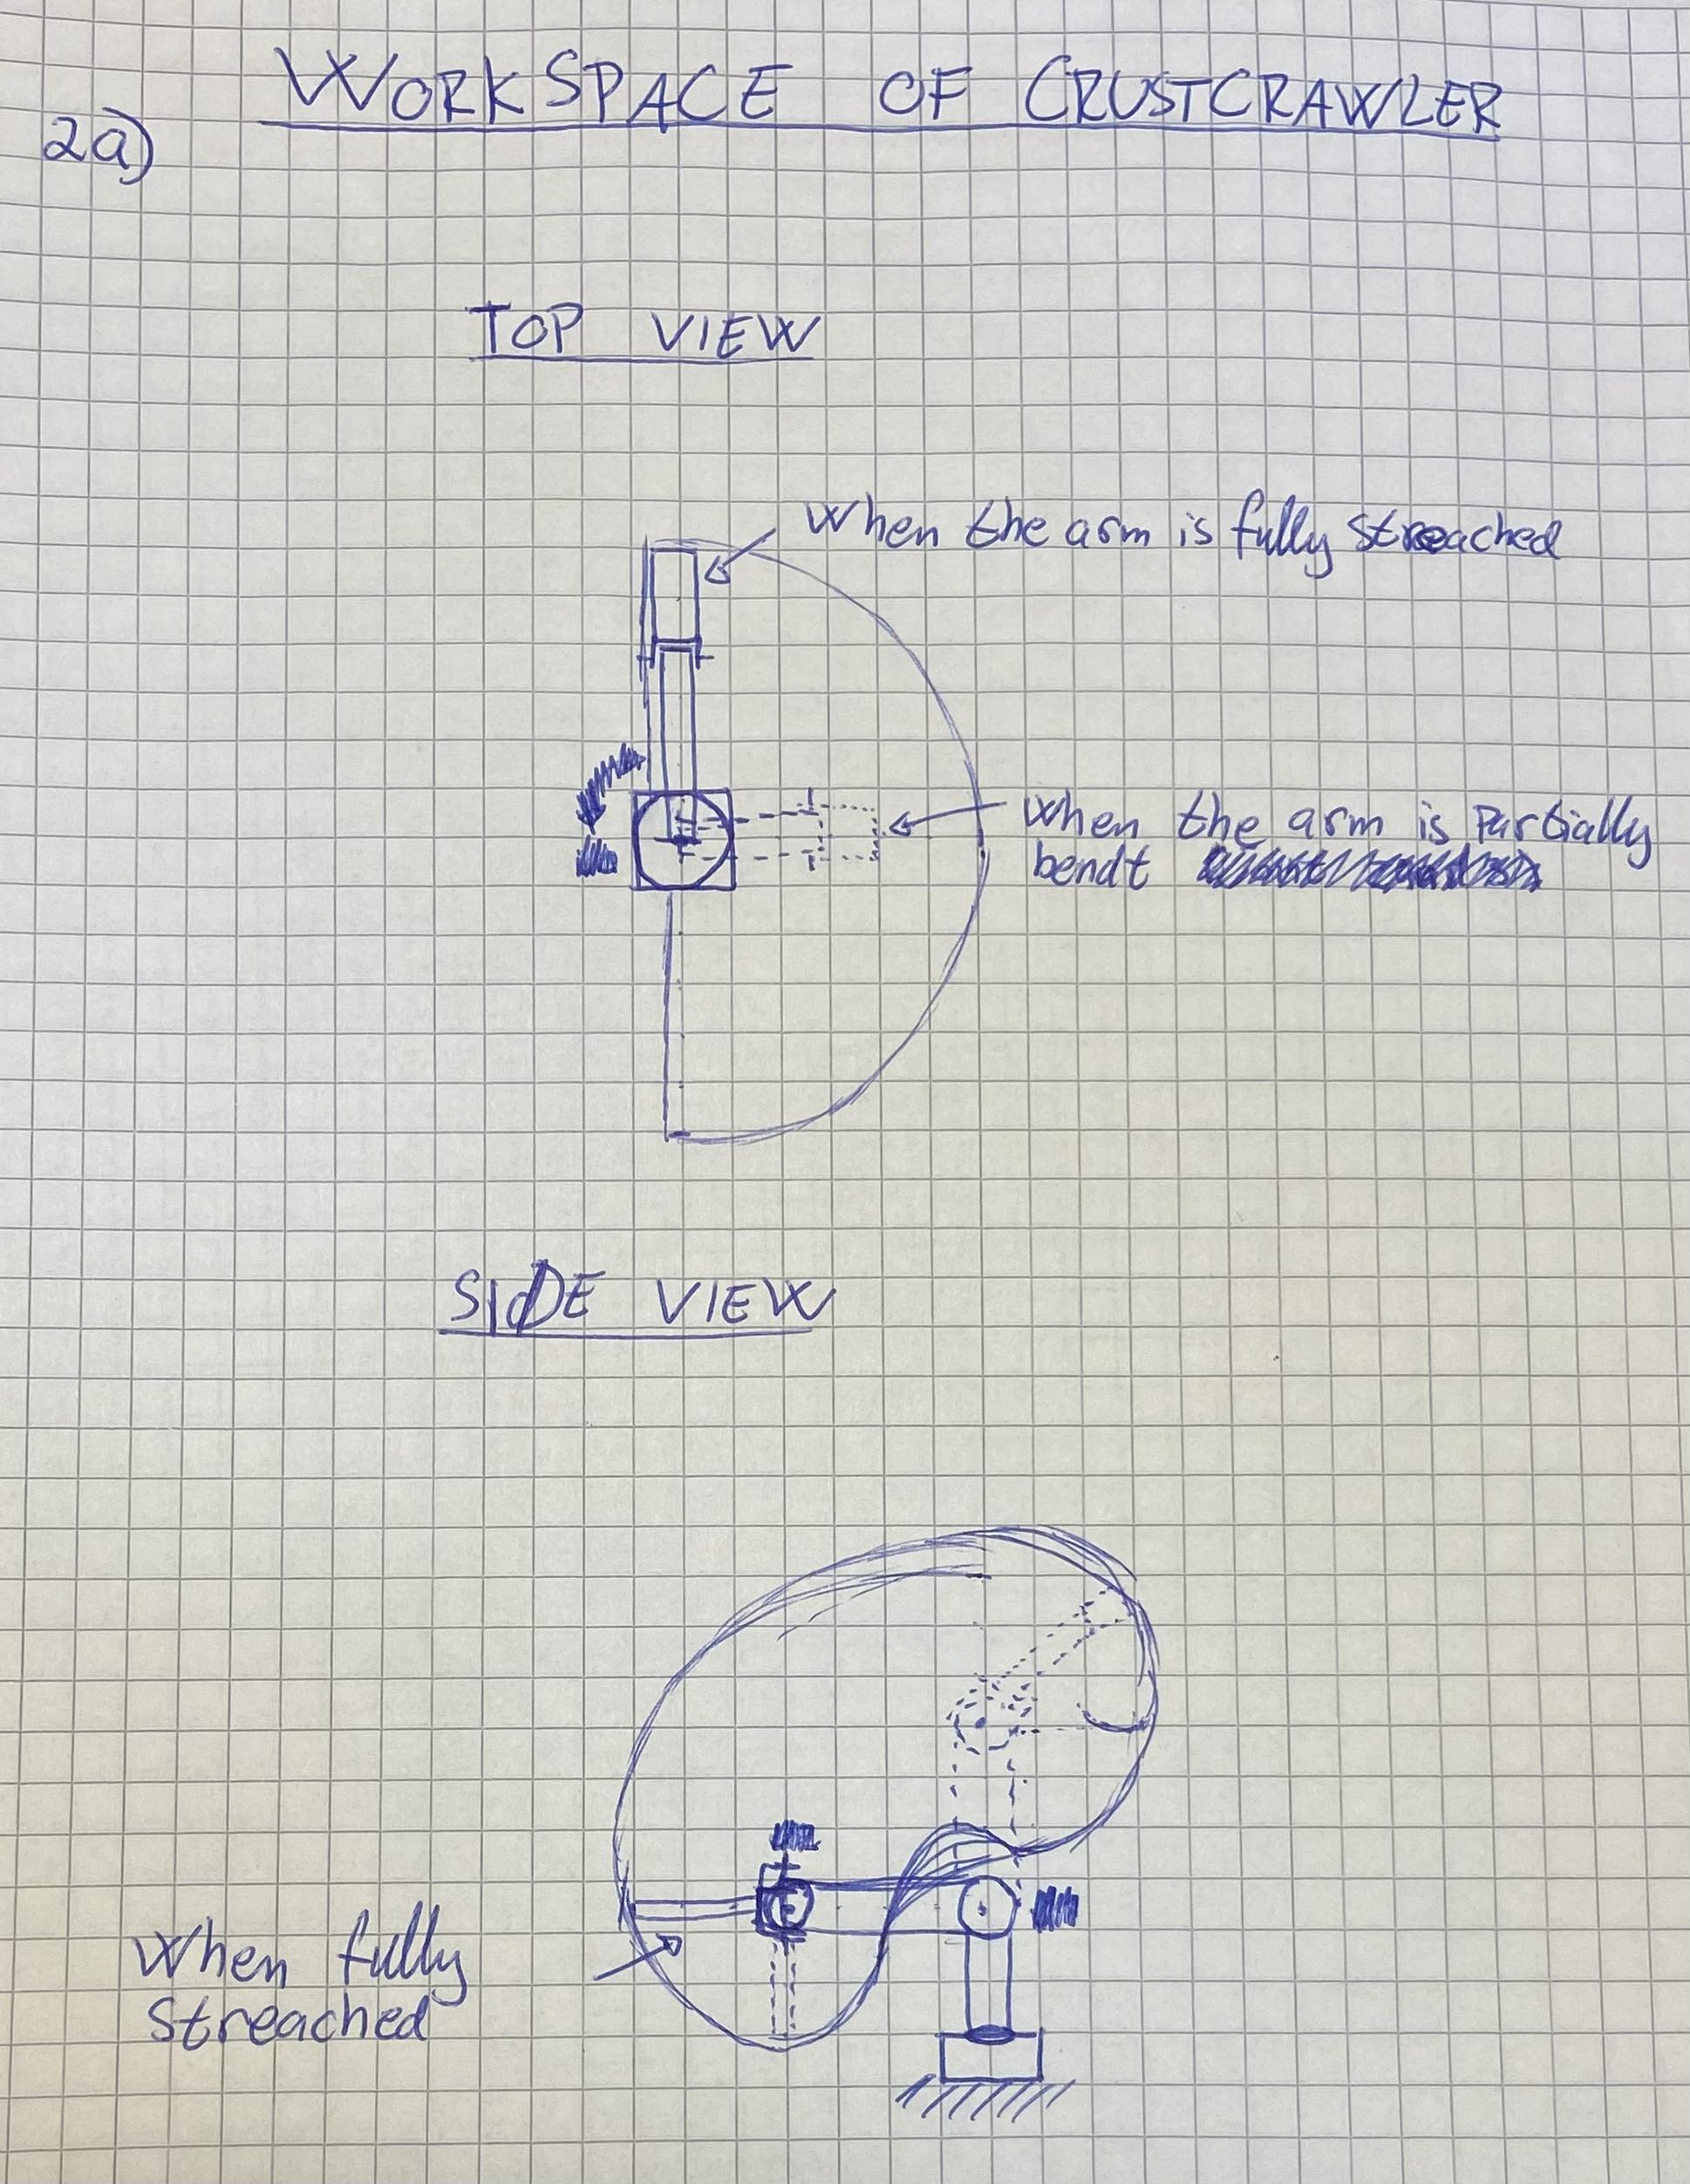
\includegraphics[width=0.6\textwidth]{workspace.jpg}\\
    I limited the joints to make clear how it affected the workspace.
    \begin{itemize}
        \item $\theta_1$ is limited to approximatly 180$^{\circ}$
        \item $\theta_2$ is limited to approximatly 90$^{\circ}$
        \item $\theta_3$ is limited to approximatly 350$^{\circ}$
    \end{itemize}
    \textbf{2b)}
    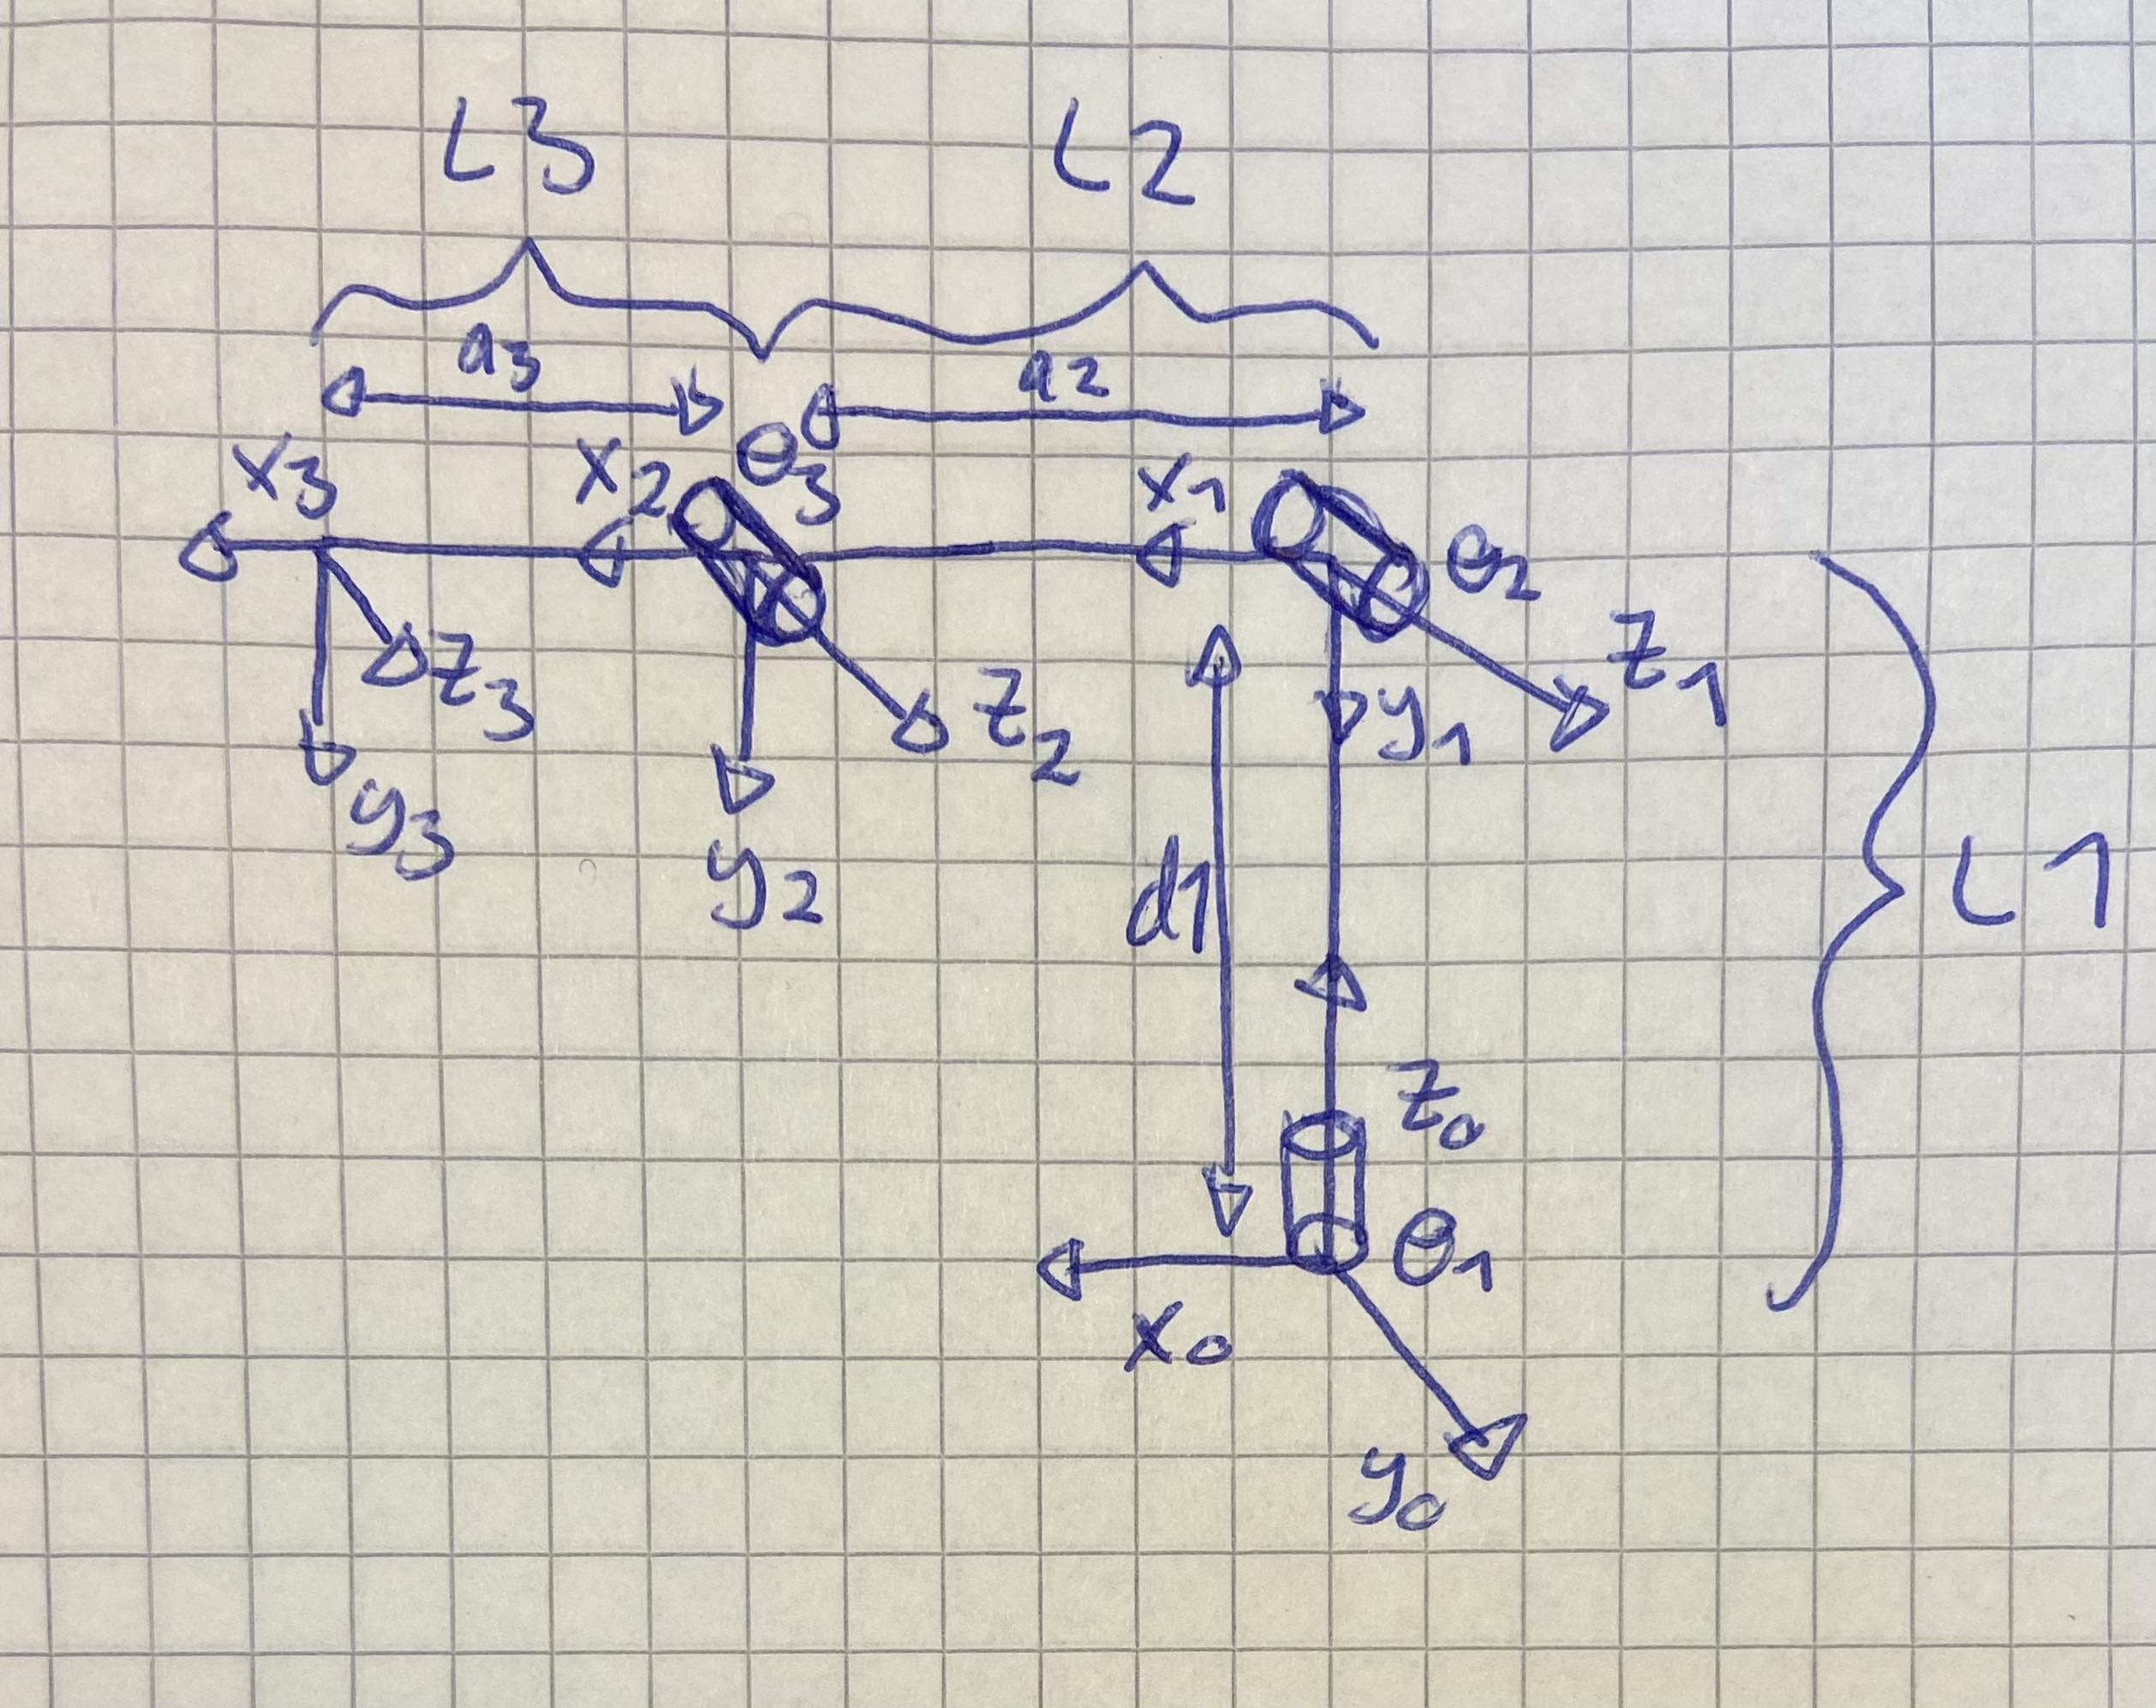
\includegraphics[width=0.7\textwidth]{NewRobot.jpg}
    \newpage
    \textbf{DH parameters:}\\
    \begin{center}
        \begin{tabular}{ c c c c c}
          & \textbf{$a_i$} & \textbf{$\alpha_i$} & \textbf{$d_i$} & \textbf{$\theta_i$}\\ 
         L1 & 0 & -90$^{\circ}$ & $d_1$ & $\theta_1*$\\  
         L2 & $a_2$ & 0 & 0 & $\theta_2*$\\
         L3 & $a_3$ & 0 & 0 & $\theta_3*$
        \end{tabular}
    \end{center}
    * means variable\\\\
    Chose to place the origin at the base of the first joint, at $0_0x_0y_0z_0$.
    Then placed $z_0$ to $z_3$ at the rotational axis of the three revolute joints. Then chose the $x_0$ arbitrarily, and placed $y_0$ according to the right hand rule.
    Chose $x_1$ to point in the direction of link 2 and parallell to $x_0$ (and perpendicular to both $z_0$ and $z_1$ to follow the convention).
    Lastly i chose the $0_2x_2y_2z_2$- and $0_3x_3y_3z_3$-coordinate system to match the previous so the numbers in the DH-table would be as easy as possible (no rotations). Then i filled in the missing y-axises.\\


    \textbf{2c)}\\
    From here $c_1$ signify $\cos(\theta_1)$, $c_2$ signify $\cos(\theta_2)$ and $c_3$ signify $\cos(\theta_3)$. And the same applies to $s_i$, where 1 $\leq$ i $\leq$ 3
   
    Calculated matrix:\\
    \[T_1T_2T_3 = 
            \left[ \begin{array}{cccc}
                c_1 & 0 & -s_1 & 0 \\
                s_1 & 0 & c_1 & 0 \\
                0 & -1 & 0 & d_1 \\
                0 & 0 & 0 & 1 \\
            \end{array} \right]
            \left[ \begin{array}{cccc}
                c_2 & -s_2 & 0 & a_2c_2 \\
                s_2 & c_2 & 0 & a_1s_2 \\
                0 & 0 & 1 & 0 \\
                0 & 0 & 0 & 1 \\
            \end{array} \right]
            \left[ \begin{array}{cccc}
                c_3 & -s_3 & 0 & a_3c_3 \\
                s_3 & c_3 & 0 & a_3s_3 \\
                0 & 0 & 1 & 0 \\
                0 & 0 & 0 & 1 \\
            \end{array} \right]\]
        

        \[= (T_1T_2)T_3 = 
        \left[ \begin{array}{cccc}
            c_1c_2 & -s_2c_1 & -s_1 & a_2c_1c_2 \\
            s_1c_2 & -s_1s_2 & c_1 & a_2s_2+d_1 \\
            -s_2 & -c_2 & 0 & -a_2s_2+d_1 \\
            0 & 0 & 0 & 1 \\
        \end{array} \right]
        \left[ \begin{array}{cccc}
            c_3 & -s_3 & 0 & a_3c_3 \\
            s_3 & c_3 & 0 & a_3s_3 \\
            0 & 0 & 1 & 0 \\
            0 & 0 & 0 & 1 \\
        \end{array} \right]\]


            \[= T_t^{B} = 
            \underline{\left[ \begin{array}{cccc}
            c_1c_2c_3-c_1s_2s_3 & -c_1c_2s_3-c_1s_2c_3 & -s_1 & a_3c_1c_2c_3-a_3c_1s_2s_3+a_2c_1c_2 \\
            s_1c_2c_3-s_1s_2s_3 & -s_1c_2s_3-s_1s_2c_3 & c_1 & a_3s_1c_2c_3-a_3s_1s_2s_3+a_2s_1c_2 \\
            -s_2c_3-c_2s_3 & s_2s_3-c_2c_3 & 0 & -a_3s_2c_3-a_3c_2s_3-a_2s_2+d_1 \\
            0 & 0 & 0 & 1 \\
            \end{array} \right]}\]


    \newpage
    \section{Task}
    Filling inn the angles:
    \begin{itemize}
        \item $\phi_1 = 270^{\circ}$ gives $\theta_1 = 270^{\circ}$ since the coordinatsystem is the same
        \item $\phi_2 = 60^{\circ}$ gives $\theta_2 = -90^{\circ}+60^{\circ} = -30^{\circ}$ because my coordinatesystem is angled 90$^{\circ}$ more in a counter clockwise direction than the configuration in the assingment (which is straight upwards)
        \item $\phi_3 = 45^{\circ}$ gives $\theta_3 = 45^{\circ}$ since when $\theta_2$ is straightened upwards, link 2 and 3 will already be angled straight upwards (in $z_0$-direction), wich makes it equal to the configuration in the assingment before the rotations
    \end{itemize}
    Filling inn the translations:
    \begin{itemize}
        \item L1 gives $d_1 = 100.9mm$
        \item L2 gives $a_2 = 222.1mm$
        \item L3 gives $a_3 = 136.2mm$
    \end{itemize}


        Coordinates of point p with respect to coordinate frame B:\\
        \[P^B = T_t^B*P^t
        = \left[ \begin{array}{cccc}
            r_{11}   &   r_{12}  &    r_{13}   &    0 \\
            r_{21}   & r_{22}    &   r_{23}    &   -227.6 \\
            r_{31}   &  r_{11}   &   r_{33}    &   343.5 \\
            0        &  0        &   0         &   1 \\
            \end{array} \right]
            \left[ \begin{array}{c}
                0\\
                0\\
                0\\
                1\\
                \end{array} \right]
        =  \left[ \begin{array}{cccc}
            0 \\
            -323.9 \\
            176.7 \\
            1 \\
            \end{array} \right]
            \]

        Coordinates of point p with respect to coordinate frame T:\\
        \[P^T = T_B^T*P^B = {(T_T^B)}^{-1}P^B
        = \left[ \begin{array}{cc}
            R^T & -R^Td \\
            0 & 1\\
            \end{array} \right]P^B
        = \left[ \begin{array}{cccc}
            0     &   1    &    0   &    750 \\
            -1   &  0    &   0    &   250 \\
            0  & 0    &   1    & -100 \\
            0     &  0     &   0    &   1 \\
            \end{array} \right]
            \left[ \begin{array}{cccc}
                0 \\
                -323.9 \\
                176.7 \\
                1 \\
                \end{array} \right]
            =\left[ \begin{array}{cccc}
                426.1 \\
                250 \\
                76.7 \\
                1 \\
                \end{array} \right]\]
        
        So the coordinates of point p in coordinatesystem T (Task) is:\\
        $p^T$ = \underline{(426.1 , 250 , 76.7)}
        \newpage
        

    \section{Task}
    \textbf{4a)}
    \begin{itemize}
        \item \textbf{Analytical approach:} You base the $x_c$-, $y_c$- and $z_c$-coordinates on the d-coloumn in the homogeneous transformation matrix (the translation). And from there you find expressions for each of the variables.
        \item \textbf{Geometrical approach:} You view the robot in different planes (two dimentions at a time). And calculate the variables that vary in that plane.
    \end{itemize}
    I will be using the analytical approach in task 4b)\\

    \textbf{4b) Analytical}\\
    \[T_t^{B} = \left[ \begin{array}{cccc}
        c_1c_2c_3-c_1s_2s_3 & -c_1c_2s_3-c_1s_2c_3 & -s_1 & a_3c_1c_2c_3-a_3c_1s_2s_3+a_2c_1c_2 \\
        s_1c_2c_3-s_1s_2s_3 & -s_1c_2s_3-s_1s_2c_3 & c_1 & a_3s_1c_2c_3-a_3s_1s_2s_3-a_2s_1c_2 \\
        -s_2c_3-c_2s_3 & s_2s_3-c_2c_3 & 0 & -a_3s_2c_3-a_3c_2s_3-a_2s_2+d_1 \\
        0 & 0 & 0 & 1 \\
        \end{array} \right]\]
    Viewing the last column:\\
    \[\left[ \begin{array}{c}
         a_3c_1c_2c_3-a_3c_1s_2s_3+a_2c_1c_2 \\
         a_3s_1c_2c_3-a_3s_1s_2s_3+a_2s_1c_2 \\
         -a_3s_2c_3-a_3c_2s_3-a_2s_2+d_1 \\
        \end{array} \right]
        = \left[\begin{array}{c}
            x_c\\y_c\\z_c
        \end{array}\right]\]
    Gives:\\
    \[x_c = a_3c_1c_2c_3-a_3c_1s_2s_3+a_2c_1c_2\]
    \[y_c = a_3s_1c_2c_3-a_3s_1s_2s_3+a_2s_1c_2 \]
    \[z_c = -a_3s_2c_3-a_3c_2s_3-a_2s_2+d_1\]

    The variables in this equations is $\theta_1$, $\theta_2$ and $\theta_3$.
    Observed that deviding $y_c$ by $x_c$ will give an expression for $\theta_1$:\\
    \[\frac{y_c}{x_c } = \frac{a_3s_1c_2c_3-a_3s_1s_2s_3+a_2s_1c_2}{a_3c_1c_2c_3-a_3c_1s_2s_3+a_2c_1c_2} = \frac{s_1(\cancel{a_3c_2c_3-a_3s_2s_3+a_2c_2})}{c_1(\cancel{a_3c_2c_3-a_3s_2s_3+a_2c_2})} = \frac{s_1}{c_1} = tan(\theta_1)\]
    \[\underline{atan2(y,x) = \theta_1}\]

    Trying to find expressions for $\theta_2$ and $\theta_3$ we can use the fact that $sin(u+v) = sin(u)cos(v) + cos(u)sin(v)$ and $cos(u+v) = cos(u)cos(v)-sin(u)sin(v)$:
    \[x_c = a_3c_1(c_2c_3-s_2s_3)+a_2c_1c_2 = a_3c_1c_{23}+a_2c_1c_2 = c_1(a_3c_{23}+a_2c_2)\]
    \[y_c = a_3s_1(c_2c_3-s_2s_3)+a_2s_1c_2 = a_3s_1c_{23}+a_2s_1c_2 = s_1(a_3c_{23}+a_2c_2)\]
    \[z_c = -a_3(s_2c_3+c_2s_3)-a_2s_2+d_1 = -a_3s_{23}-a_2s_2+d_1\]

    If we square $x_c$, $y_c$ and $z_c$ we can try to use the identity $c^2+s^2 = 1$. And if we move $d_1$ in the $z_1$-expression, the calculations will be easier:
    \[x_c^2 = c_1^2(a_3c_{23}+a_2c_2)^2\]
    \[y_c^2 = s_1^2(a_3c_{23}+a_2c_2)^2\]
    \[(z_c-d_1)^2 = (-a_3s_{23}-a_2s_2)^2\]
  
    Adding $x_c^2$ and $y_c^2$ together:
    \[x_c^2+y_c^2 = c_1^2(a_3c_{23}+a_2c_2)^2 + s_1^2(a_3c_{23}+a_2c_2)^2 = (\cancel{c_1^2+s_1^2})(a_3c_{23}+a_2c_2)^2 = (a_3c_{23}+a_2c_2)^2\]
    
    Adding in the $(z_c-d_1)^2$:
    \[x_c^2+y_c^2+(z_c-d_1)^2 = (a_3c_{23}+a_2c_2)^2+(-a_3s_{23}-a_2s_2)^2\]
    \[=a_3^2c_{23}^2+2a_2a_3c_2c_{23}+a_2^2c_2^2 + a_3^2s_{23}^2 +2a_2a_3s_2s_{23}+ a_2^2s_2^2\]
    \[=a_3^2(\cancel{c_{23}^2+s_{23}^2})+ 2a_2a_3c_2c_{23}+2a_2a_3s_2s_{23} + a_2^2(\cancel{c_2^2+s_2^2})\]
    \[=a_3^2 + 2a_2a_3c_2c_{23}+2a_2a_3s_2s_{23} + a_2^2\]

    From here we can write $c_{uv}$ out as $cos(u)cos(v) -sin(u)sin(v)$ and $s_{uv}$ as $sin(u)cos(v) + cos(u)sin(v)$\\
    \[=a_3^2 + 2a_2a_3c_2(c_2c_3-s_2s_3)+2a_2a_3s_2(s_2c_3+c_2s_3) + a_2^2\]
    \[=a_3^2 + 2a_2a_3c_2^2c_3-\cancel{2a_2a_3c_2s_2s_3}+2a_2a_3s_2^2c_3+\cancel{2a_2a_3s_2c_2s_3} + a_2^2\]
    \[=a_3^2 + 2a_2a_3c_3(\cancel{c_2^2+s_2^2})+ a_2^2\]
    \[=a_3^2 + 2a_2a_3c_3+ a_2^2\]

    This expression has only one variable ($\theta_3$), which gives:
    \[x_c^2+y_c^2+(z_c-d_1)^2=a_3^2 + 2a_2a_3c_3+ a_2^2\]
    \[2a_2a_3c_3 = x_c^2+y_c^2+(z_c-d_1)^2-a_3^2-a_2^2\]
    \[c_3 = cos(\theta_3) = \frac{x_c^2+y_c^2+(z_c-d_1)^2-a_3^2-a_2^2}{2a_2a_3} := D\]
    
    To find a singular and defined value for all $\theta_3$ we use arctan2 and expression D:
    \[s_3 = \pm\sqrt{1-c_3^2} = \pm\sqrt{1-D^2}\]
    \[tan(\theta_3) = \frac{s_3}{c_3} = \frac{\pm\sqrt{1-D^2}}{D}\]
    \[\theta_3 = atan2(\pm\sqrt{1-D^2}, D)\]

    And then the only missing variable is $\theta_2$, so we try to make the $x_c$-expression on the form $acos\theta+bsin\theta= c$
    so that $\theta$ can be found by the formula $\theta$ = $atan2(\frac{b}{a})\pm atan2(\frac{\sqrt{a^2+b^2+c^2}}{c})$:
    \[x_c = a_3c_1c_2c_3-a_3c_1s_2s_3+a_2c_1c_2\]
    \[x_c = (a_3c_1c_3+a_2c_1)c_2+(-a_3c_1s_3)s_2\]
    To fill inn the formula: $a = a_3c_1c_3+a_2c_1$, $b= -a_3c_1s_3$ and $c = x_c$:
    \[\theta_2 = \underline{atan2(\frac{-a_3c_1s_3}{a_3c_1c_3+a_2c_1})\pm atan2(\frac{\sqrt{(a_3c_1c_3+a_2c_1)^2+(-a_3c_1s_3)^2+x_c^2}}{x_c})}\]

    \textbf{4c)}\\
    Number of solutions for different positions of the tip (of link 3):
    \begin{itemize}
        \item \textbf{1 if the tip of link 3 is at the border of workspace (except special case*)}\\
        Because to reach the outer border, link 3 must be an extention of link 2 (streached out).
        The border of workspace can also be reached if link 2 and 3 are extentions of link 1, but this is a special case (defined under).
        \item \textbf{2 if the tip of link 3 is in the workspace (except special case*)}\\
        $\theta_2$ and $\theta_3$ can vary by making the elbow down or elbow up.
        \item \textbf{*$\infty$ if the tip of link 3 intersects the $z_0$-axis}\\
        In this special case the angle of $\theta_1$ does not matter. So it can rotate 365 degrees, 
        and the tip of link 3 will still be at the same position.
    \end{itemize}


        
\end{document}